\documentclass{standalone}
\usepackage{hsbcommon}
\begin{document}
    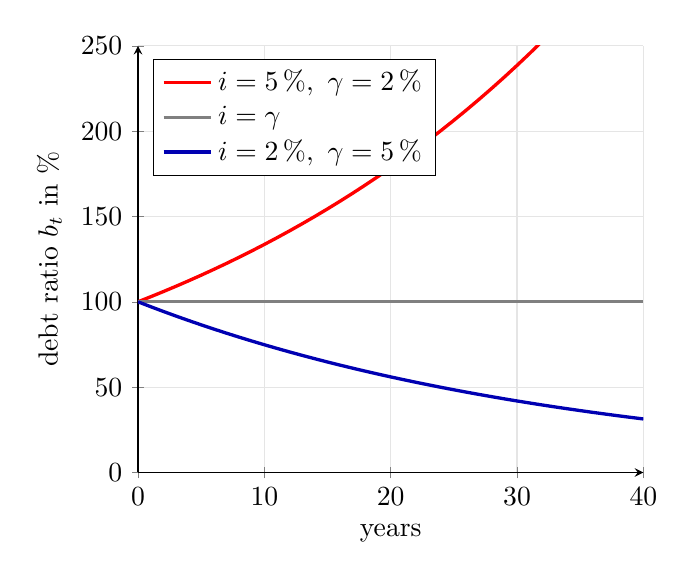
\begin{tikzpicture}
        \begin{axis}[
          width=8cm, height=7cm,
          xmin=0, xmax=40, ymin=0, ymax=250,
          xlabel={years}, ylabel={debt ratio $b_t$ in \%},
          axis lines=left, grid=major, grid style={gray!20},
          legend pos=north west, legend cell align=left,
          domain=0:40, samples=41,
        ]
        \addplot[very thick, red] {100*(1.05/1.02)^x};
        \addlegendentry{$i=5\,\%,\ \gamma=2\,\%$}
        \addplot[very thick, gray] {100};
        \addlegendentry{$i=\gamma$}
        \addplot[very thick, blue!70!black] {100*(1.02/1.05)^x};
        \addlegendentry{$i=2\,\%,\ \gamma=5\,\%$}
        \end{axis}
    \end{tikzpicture}
\end{document}